\documentclass[9pt,twocolumn,twoside]{pnas-new}
\usepackage{verbatim}
% Use the lineno option to display guide line numbers if required.
% Note that the use of elements such as single-column equations
% may affect the guide line number alignment. 

\templatetype{pnasmathematics} % Choose template 
% {pnasresearcharticle} = Template for a two-column research article
% {pnasmathematics} = Template for a one-column mathematics article
% {pnasinvited} = Template for a PNAS invited submission

\title{Energy analysis and predictive modeling to investigate renewable energy trends in the states of Arizona, California, New Mexico, and Texas }

% Use letters for affiliations, numbers to show equal authorship (if applicable) and to indicate the corresponding author
\author{Richard Carini}
\author{Nicholas Geis} 
\author{Matthew Uffenheimer}

\affil{University of California, Santa Barbara, Mathematics Department}


% Please give the surname of the lead author for the running footer
%\leadauthor{Lead author last name} 

% Please add here a significance statement to explain the relevance of your work

% Please include corresponding author, author contribution and author declaration information
%\authorcontributions{Please provide details of author contributions here.}
%\authordeclaration{Please declare any conflict of interest here.}
%\equalauthors{\textsuperscript{1}A.O.(Author One) and A.T. (Author Two) contributed equally to this work (remove if not applicable).}
%\correspondingauthor{\textsuperscript{2}To whom correspondence should be addressed. E-mail: author.two\@email.com}

% Keywords are not mandatory, but authors are strongly encouraged to provide them. If provided, please include two to five keywords, separated by the pipe symbol, e.g:
%\keywords{Keyword 1 $|$ Keyword 2 $|$ Keyword 3 $|$ ...} 

\begin{abstract}
Please provide an abstract of no more than 250 words in a single paragraph. Abstracts should explain to the general reader the major contributions of the article. References in the abstract must be cited in full within the abstract itself and cited in the text.
\end{abstract}

\dates{This manuscript was compiled on \today}

\begin{document}

% Optional adjustment to line up main text (after abstract) of first page with line numbers, when using both lineno and twocolumn options.
% You should only change this length when you've finalised the article contents.
\verticaladjustment{-2pt}

\maketitle
\thispagestyle{firststyle}
\ifthenelse{\boolean{shortarticle}}{\ifthenelse{\boolean{singlecolumn}}{\abscontentformatted}{\abscontent}}{}

% If your first paragraph (i.e. with the \dropcap) contains a list environment (quote, quotation, theorem, definition, enumerate, itemize...), the line after the list may have some extra indentation. If this is the case, add \parshape=0 to the end of the list environment.
\dropcap{T}his PNAS journal template is provided to help you write your work in the correct journal format.  Instructions for use are provided below.

Note: please start your introduction without including the word ``Introduction'' as a section heading (except for math articles in the Physical Sciences section); this heading is implied in the first paragraphs. 

\section*{Quick Graphs}

\begin{center}
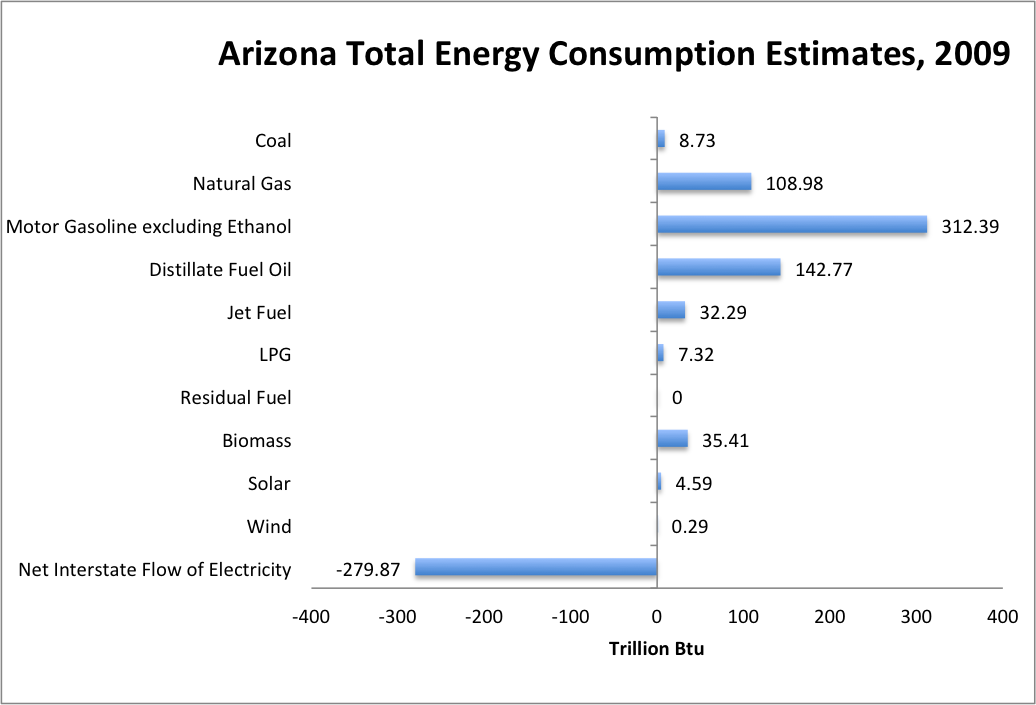
\includegraphics[width=15cm]{ArizonaQuickGraph.png}
\end{center}
\begin{center}
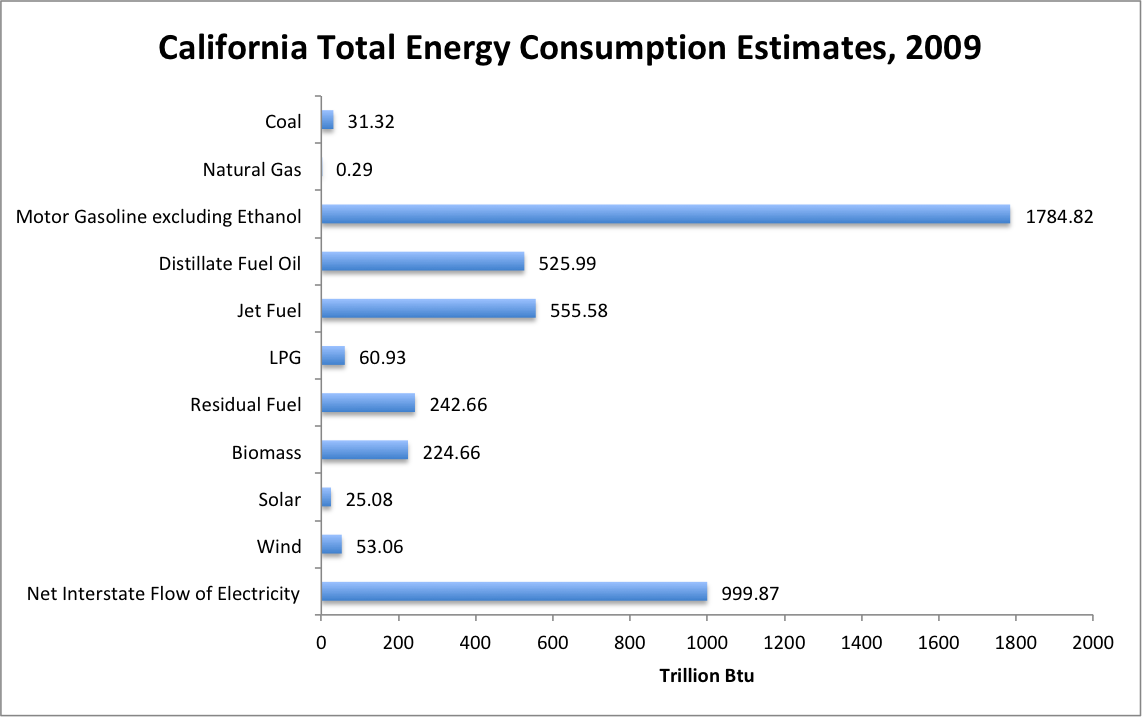
\includegraphics[width=15cm]{CaliforniaQuickGraph.png}
\end{center}
\begin{center}
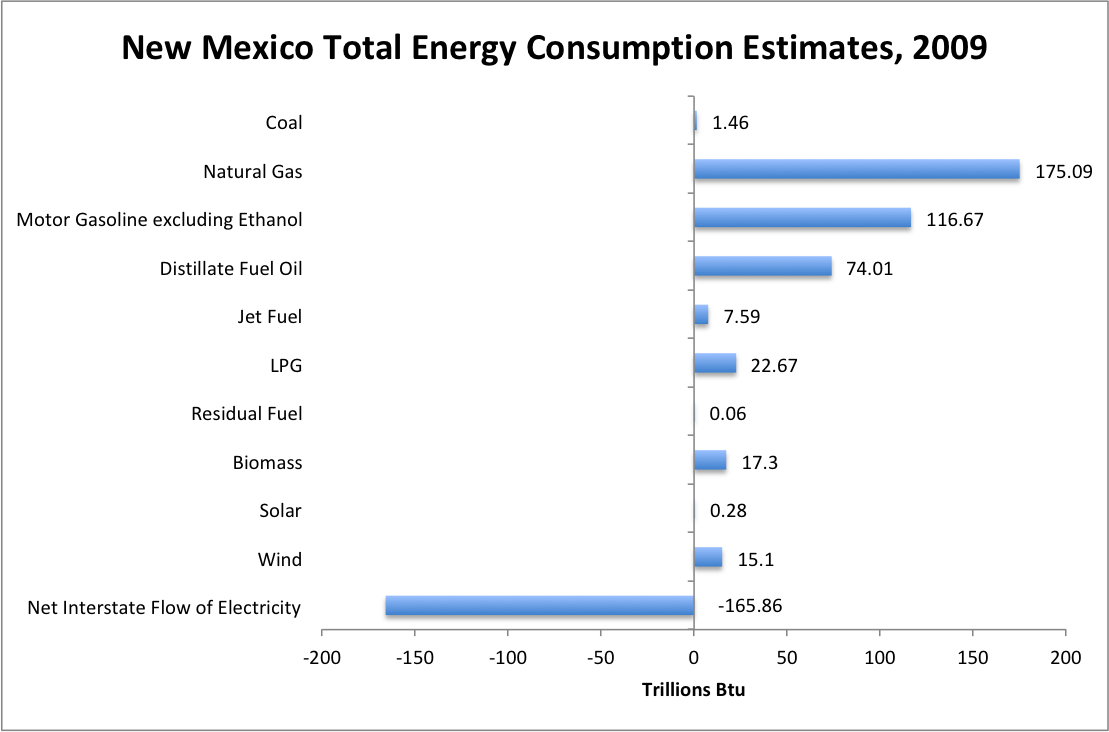
\includegraphics[width=15cm]{NewMexicoQuickGraph.png}
\end{center}
\begin{center}
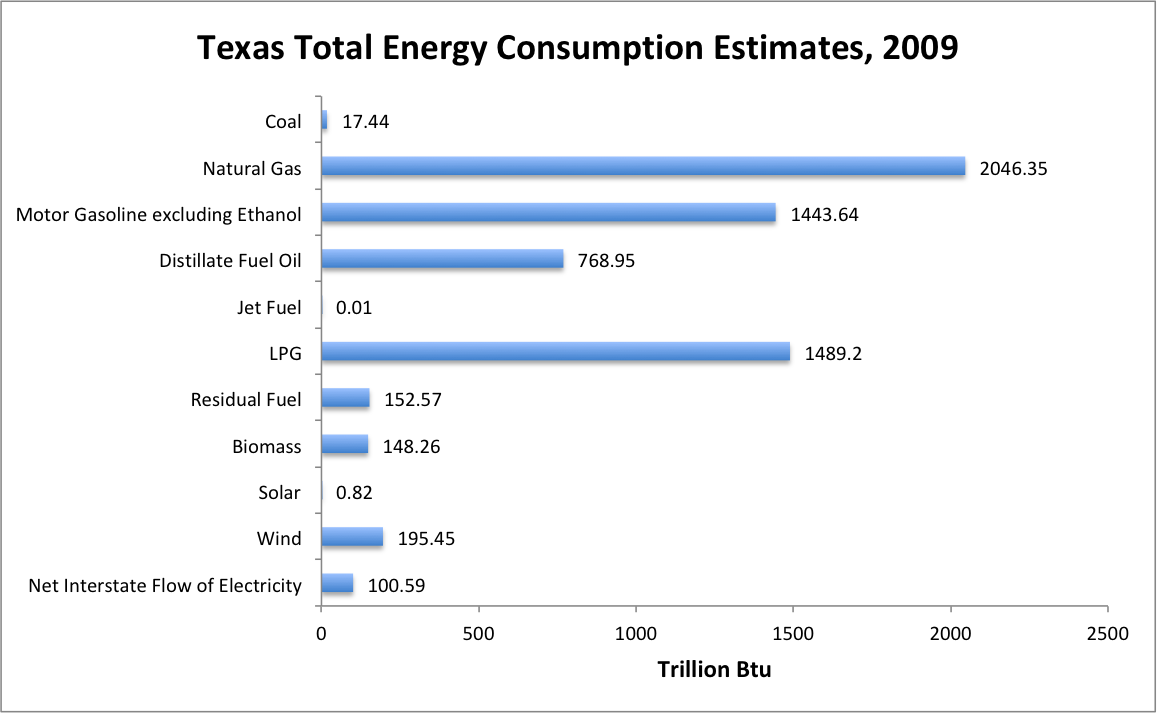
\includegraphics[width=15cm]{TexasQuickGraph.png}
\end{center}

\section*{State Information}


\subsection*{Arizona}

\begin{itemize}
\item Geography
\begin{itemize}
\item Northeastern 2/5 consists mainly of plains, mesas, and plateaus
\item Grand Canyon
\item Volcanic, forest-covered mountains 
\end{itemize}
\item Resources/Industry
\begin{itemize}
\item Coal from Black Mesa area of Native American reservations — coal-fired stations generate much of the electricity for the southwestern United States
\item Petroleum and large amounts of uranium from northeastern area
\item Strong lumber/pulp-paper industry
\end{itemize}
\item Population
\begin{itemize}
\item  “In the early 21st century Arizona’s population experienced dramatic growth at almost three times the national rate.”
\item The overall population was projected to reach 10 million by the year 2027.
\end{itemize}
\item Climate
\begin{itemize}
\item 1/2 semiarid, 1/3 arid, remainder humid
\item “Most of the region receives from 10 to 15 inches (250 to 375 mm) of precipitation annually, with the Mogollon Rim and White Mountains receiving the state’s largest average, 25 inches (625 mm).”
\end{itemize}
\item Special notes
\begin{itemize}
\item “Altogether, nearly a dozen dams control the Mogollon Rim’s runoff, impounding and diverting the water to provide flood control and lakes for water storage. This hydrologic pattern has been a source of much political and legal trouble for Arizona, including years of litigation with California over rights to water from the Colorado River system. The state’s internal sharing of water is also a major problem because groundwater has been depleted, particularly around Phoenix and Tucson, and there are no new sources of surface water. Cities have found it necessary to buy water rights from distant areas, and litigation involving municipalities, Native American tribes, and federal agencies over water rights is increasingly common.”
\end{itemize}

\end{itemize}

\subsection*{California}

\begin{itemize}
\item Geography
\begin{itemize}
\item Great physical contrasts (rainy northern coast and southern deserts)
\item Most of eastern CA is desert (Mojave Desert 1/6 of land area of CA)
\end{itemize}

\item Resources/Industry
\begin{itemize}
\item Economy is largest of any U.S. state
\item “New Economy”: leading focus on technology and computer/software service industry
\end{itemize}

\item Population
\begin{itemize}
\item Concentrated mostly along coast
\item Most urban in the United States (3/4 of population live in LA, SF, and SD)
\end{itemize}

\item Climate
\begin{itemize}
\item Water chronically scarce in Southern CA - excess rain/snowmelt cause winter flooding along rivers
\item Marked by 2 seasons: wet and dry
\item Precipitation > 170” in northwest to traces in southeast desert; moderate coast
\item Summer temp in Colorado Desert can reach 130F
\end{itemize}

\item Special notes
\begin{itemize}
\item Colorado River Aqueduct at the Arizona border carries water from that river across the southern California desert and mountains to serve the Los Angeles metropolitan area
\item The California State Water Project, launched in 1960, is the largest water-transfer system ever undertaken — designed to deliver water daily from the Feather River (a tributary of the Sacramento River) in north-central California to communities as far south as the Mexican border
\item  \url{http://www.latimes.com/projects/la-fi-electricity-solar/ }
\end{itemize}
\end{itemize}


\subsection*{New Mexico}

\begin{itemize}
\item Geography
\begin{itemize}
\item Mainly high plateaus or mesas, several mountain ranges, canyons, and valleys
\end{itemize}

\item Resources/Industry
\begin{itemize}
\item “Principal industries of New Mexico are agriculture, mining, lumbering, gas and oil production, and recreation.”
\end{itemize}

\item Population
\begin{itemize}
\item Population increase was one of the slowest in the nation from 2010-2017 -- Can't be part of final report
\end{itemize}

\item Climate
\begin{itemize}
\item “New Mexico has a mild, arid or semiarid, continental climate characterized by light precipitation totals, abundant sunshine, low relative humidities, and a relatively large annual and diurnal temperature range.”
\end{itemize}

\item Special notes
\begin{itemize}
\item The prices of oil after 2009 decreased dramatically, causing strain on the economic and governmental budget for the state since the production of oil and fuel is one of the largest in the nation. -- Can't be part of final report
\end{itemize}

\end{itemize}

\subsection*{Texas}

\begin{itemize}
\item Geography
\begin{itemize}
\item Coastal Plains encompass about 2/5 of land area
\item “In 1913 there were only 8 major lakes or reservoirs in Texas; by the early 21st century there were about 200, many of which were created to store water against periodic droughts.”
\item “The North Plains subdivision, centered on Amarillo, depends on grain farming, ranching, oil, and small industries.”
\end{itemize}

\item Resources/Industry
\begin{itemize}
\item "Texas leads all other states in oil and natural gas production. It also ranks first in oil-refining capacity. Oil deposits have been found under more than two-thirds of the state’s area, though many finds have been too small for commercial development. The Gulf Coast area is the centre for the state’s petrochemical industrial complexes.”
\item “Texas economy has remained heavily dependent on oil and gas, and any fluctuations in oil prices have had a major impact on the state.”
\end{itemize}

\item Population
\begin{itemize}
\item “Access to water transportation, reservoirs of natural gas and oil, and availability of raw materials have made the coastal area the centre of industry in Texas. “

\end{itemize}

\item Climate
\begin{itemize}
\item “January temperatures in the Rio Grande valley have been known to register well into the 90s F, while blizzards have blocked highways in the Panhandle section of the state during the same month” — fluctuations in weather patterns creates high/low pressure densities, ideal for wind/storm formation
\item Gulf coast of Texas especially prone to hurricanes
\end{itemize}

\item Special notes
\begin{itemize}
\item “Texas leads the country in the production of wind energy and generates about one-third of total U.S. wind capacity. Most of the state’s wind turbines are located in the Panhandle and in the Trans-Pecos region. One of the largest wind farms in the world, the Horse Hollow Wind Energy Center, is spread across some 50,000 acres (20,000 hectares) near Abilene.”
\item “Other renewable sources of growing importance in Texas are solar and geothermal energy.”

\end{itemize}

\end{itemize}

\subsection*{Similarities and Differences Summary}
\begin{itemize}
\item Geography: Arizona and New Mexico of similar size; contains mostly plateaus and mesas. Texas has incredibly large amount of area in Coastal Plains - used for oil \& petrochemical industries (convert towards solar/geothermal?). California large coastal region (a lot of hydro opportunities?). Smaller sizes/smaller urban areas of NM and AZ may cause lower road oil consumed by transportation compared to CA and TX

\item Resources/Industry: Texas and New Mexico leaders in oil and natural gas. Arizona large amounts of coal reserves. California has incredibly large economy due to leading the software and computing industry: potential for investment in pricier forms of alternative energies(?). Texas's technology industry also on the rise - may follow suit in the future(?)

\item Population: look at data sets that we have to interpret data

\item Climate: Arizona and New Mexico similar in terms of being arid and dry; California and Texas more diverse climates overall, Texas more diverse in smaller areas - may be cause of strong wind energy production.
\end{itemize}

\section*{References}

Britannica \url{ https://www.britannica.com/place/Texas-state}\\
\url{https://wrcc.dri.edu/narratives/NEWMEXICO.htm}

\begin{comment}
\subsection*{Data Archival}

PNAS must be able to archive the data essential to a published article. Where such archiving is not possible, deposition of data in public databases, such as GenBank, ArrayExpress, Protein Data Bank, Unidata, and others outlined in the Information for Authors, is acceptable.

\subsection*{Language-Editing Services}
Prior to submission, authors who believe their manuscripts would benefit from professional editing are encouraged to use a language-editing service (see list at www.pnas.org/site/authors/language-editing.xhtml). PNAS does not take responsibility for or endorse these services, and their use has no bearing on acceptance of a manuscript for publication. 

\subsection*{Digital Figures}
\label{sec:figures}

Only TIFF, EPS, and high-resolution PDF for Mac or PC are allowed for figures that will appear in the main text, and images must be final size. Authors may submit U3D or PRC files for 3D images; these must be accompanied by 2D representations in TIFF, EPS, or high-resolution PDF format.  Color images must be in RGB (red, green, blue) mode. Include the font files for any text. 

Figures and Tables should be labelled and referenced in the standard way using the \verb|\label{}| and \verb|\ref{}| commands.

Figure \ref{fig:frog} shows an example of how to insert a column-wide figure. To insert a figure wider than one column, please use the \verb|\begin{figure*}...\end{figure*}| environment. Figures wider than one column should be sized to 11.4 cm or 17.8 cm wide. Use \verb|\begin{SCfigure*}...\end{SCfigure*}| for a wide figure with side captions.

\subsection*{Single column equations}

Authors may use 1- or 2-column equations in their article, according to their preference.

To allow an equation to span both columns, options are to use the \verb|\begin{figure*}...\end{figure*}| environment mentioned above for figures, or to use the \verb|\begin{widetext}...\end{widetext}| environment as shown in equation \ref{eqn:example} below.

Please note that this option may run into problems with floats and footnotes, as mentioned in the \href{http://texdoc.net/pkg/cuted}{cuted package documentation}. In the case of problems with footnotes, it may be possible to correct the situation using commands \verb|\footnotemark| and \verb|\footnotetext|.

%% Do not use widetext if paper is in single column.
\begin{widetext}
\begin{align*}
(x+y)^3&=(x+y)(x+y)^2\\
       &=(x+y)(x^2+2xy+y^2) \numberthis \label{eqn:example} \\
       &=x^3+3x^2y+3xy^3+x^3. 
\end{align*}
\end{widetext}

\begin{table}%[tbhp]
\centering
\caption{Comparison of the fitted potential energy surfaces and ab initio benchmark electronic energy calculations}
\begin{tabular}{lrrr}
Species & CBS & CV & G3 \\
\midrule
1. Acetaldehyde & 0.0 & 0.0 & 0.0 \\
2. Vinyl alcohol & 9.1 & 9.6 & 13.5 \\
3. Hydroxyethylidene & 50.8 & 51.2 & 54.0\\
\bottomrule
\end{tabular}

\addtabletext{nomenclature for the TSs refers to the numbered species in the table.}
\end{table}

\subsection*{Supporting Information (SI)}

The main text of the paper must stand on its own without the SI. Refer to SI in the manuscript at an appropriate point in the text. Number supporting figures and tables starting with S1, S2, etc. Authors are limited to no more than 10 SI files, not including movie files. Authors who place detailed materials and methods in SI must provide sufficient detail in the main text methods to enable a reader to follow the logic of the procedures and results and also must reference the online methods. If a paper is fundamentally a study of a new method or technique, then the methods must be described completely in the main text. Because PNAS edits SI and composes it into a single PDF, authors must provide the following file formats only.

\subsubsection*{SI Text}

Supply Word, RTF, or LaTeX files (LaTeX files must be accompanied by a PDF with the same file name for visual reference).

\subsubsection*{SI Figures}

Provide a brief legend for each supporting figure after the supporting text. Provide figure images in TIFF, EPS, high-resolution PDF, JPEG, or GIF format; figures may not be embedded in manuscript text. When saving TIFF files, use only LZW compression; do not use JPEG compression. Do not save figure numbers, legends, or author names as part of the image. Composite figures must be pre-assembled.

\subsubsection*{3D Figures}

Supply a composable U3D or PRC file so that it may be edited and composed. Authors may submit a PDF file but please note it will be published in raw format and will not be edited or composed.

\subsubsection*{SI Tables}

Supply Word, RTF, or LaTeX files (LaTeX files must be accompanied by a PDF with the same file name for visual reference); include only one table per file. Do not use tabs or spaces to separate columns in Word tables.

\subsubsection*{SI Datasets} 

Supply Excel (.xls), RTF, or PDF files. This file type will be published in raw format and will not be edited or composed. 

\subsubsection*{SI Movies}

Supply Audio Video Interleave (avi), Quicktime (mov), Windows Media (wmv), animated GIF (gif), or MPEG files and submit a brief legend for each movie in a Word or RTF file. All movies should be submitted at the desired reproduction size and length. Movies should be no more than 10 MB in size. 

\subsubsection*{Still images}

Authors must provide a still image from each video file. Supply TIFF, EPS, high-resolution PDF, JPEG, or GIF files. 

\subsubsection*{Appendices}

PNAS prefers that authors submit individual source files to ensure readability. If this is not possible, supply a single PDF file that contains all of the SI associated with the paper. This file type will be published in raw format and will not be edited or composed.

\matmethods{Please describe your materials and methods here. This can be more than one paragraph, and may contain subsections and equations as required. Authors should include a statement in the methods section describing how readers will be able to access the data in the paper. 

\subsection*{Subsection for Method}
Example text for subsection.
}

\showmatmethods{} % Display the Materials and Methods section

\acknow{Please include your acknowledgments here, set in a single paragraph. Please do not include any acknowledgments in the Supporting Information, or anywhere else in the manuscript.}

\showacknow{} % Display the acknowledgments section

% \pnasbreak splits and balances the columns before the references.
% Uncomment \pnasbreak to view the references in the PNAS-style
% If you see unexpected formatting errors, try commenting out \pnasbreak
% as it can run into problems with floats and footnotes on the final page.
%\pnasbreak

\end{comment}

% Bibliography
\bibliography{pnas-sample}

\end{document}